\section{Testing}
\subsection{Modultest Game Engine}
Denne modultest har til formål at teste Game Engine, for at sikre at Spillet
funktionaliteter afvilket på korrekt vis men spillet spilles. Der er gjort
stor brug af Robert C. Martins ``Three Laws of TDD'' \parencite[Side 122]{CleanCode}.

I tilfælde som GameController, Players og andre klasser, som er afhængige af 
eksempelvis DiceRoller eller andre klasser, er der blevet brugt mocks og
dependency injections til at dække alle senarier som det ses \autoref{fig:mock}.

Dependencies til DiceRoller har især krævet mocks da denne ellers genererer 
psudo-random tal hvilket gør det umuligt at test andre komponenter, som er 
afhængig af specifikke outputs for teste en specifik opførsel.

\newpage 

\subsubsection{GodkendelsesTabel Game Engine}
\captionof{table}{Her Ses en komplet liste over alle test foretages på
                  Game Engine komponenter, med kommentar til deres resultater
                  og en endelig vurdering af test resultaterne.}
\vspace{-1em}
\begin{center}
\begin{longtable}{|l|p{0.25\linewidth}|p{0.25\linewidth}|l|}
  \hline
  \multicolumn{4}{|c|}{\textbf{Game Engine GodkendelsesTabel}} \\ \hline
  \textbf{Komponent under test} & \textbf{Forventet Adfærd} & \textbf{Kommentar} & \textbf{Test Resultat} \\ \hline
  Game Controller
  &
    \begin{enumerate}
      \item \begin{flushleft} Kan skifte Player til Nyt Room \end{flushleft}
      \item \begin{flushleft} Kan samle Item op fra Room  \end{flushleft}
      \item \begin{flushleft} Kan save Game \end{flushleft}
      \item \begin{flushleft} Kan loaded Games \end{flushleft}
      \item \begin{flushleft} Kan eliminere Enemy fra Game \end{flushleft}
      \item \begin{flushleft} Kan reset Game \end{flushleft}
      \item \begin{flushleft} Kan anskaffe Room description \end{flushleft}
    \end{enumerate}
  &
  \flushleft 
  Game Controller Har kun test for at skifte til nyt Room
  &
  FAIL
  \\ \hline
  Combat Controller
  &
  \begin{enumerate}
    \item \begin{flushleft} Kan Håndtere Combat Rounds \end{flushleft}
    \item \begin{flushleft} Kan håndtere at Player løber væk fra Combat \end{flushleft}
  \end{enumerate}
  &
  \flushleft
  Combat controller kan håndtere at spilleren løber fra combat og at Player engager i combat.
  &
  OK
  \\ \hline
  DiceRoller
  &
  \begin{enumerate}
    \item \begin{flushleft} Kan emulerer et kast med en N siddet terning \end{flushleft}
    \item \begin{flushleft} Kan emulerer N kast med en M siddet terning \end{flushleft}
  \end{enumerate}
  &
  \flushleft
  DiceRoller Kan emulere et eller flere terninge kast med samme antal sidder.
  &
  OK
  \\ \hline
  BaseMapCreator
  &
  \begin{enumerate}
    \item \begin{flushleft} Kan generere et map layout file \end{flushleft}
  \end{enumerate}
  &
  \flushleft
  BaseMapCreator can på korrekt vis generere et map layout file
  &
  OK
  \\ \hline
  BaseMap
  &
  \begin{enumerate}
    \item \begin{flushleft} Kan anskaffe Rooms ud fra en Direction \end{flushleft}
  \end{enumerate}
  &
  \flushleft
  Map kan anskaffe Rooms uf fra en given Direction.
  &
  OK
  \\ \hline
  Player
  &
  \begin{enumerate}
    \item \begin{flushleft} Kan angribe Enemy  \end{flushleft}
    \item \begin{flushleft} Kan tage skade \end{flushleft}
    \item \begin{flushleft} Kan skade Enemy (Ikke Kristisk)  \end{flushleft}
    \item \begin{flushleft} Kan skade Enemy (Kritisk)  \end{flushleft}
  \end{enumerate}
  &
  \flushleft
  Player kan angribe, skade og tage skade fra enemy.
  &
  OK
  \\ \hline
  Enemy
  &
  \begin{enumerate}
    \item \begin{flushleft} Kan angribe Player  \end{flushleft}
    \item \begin{flushleft} Kan tage skade \end{flushleft}
    \item \begin{flushleft} Kan skade Player (Ikke Kristisk)  \end{flushleft}
    \item \begin{flushleft} Kan skade Player (Kritisk)  \end{flushleft}
  \end{enumerate}
  &
  \flushleft
  Enemy kan angribe, skade og tage skade fra Player.
  &
  OK
  \\ \hline
  Log
  &
  \begin{enumerate}
    \item \begin{flushleft} Kan log et event \end{flushleft}
    \item \begin{flushleft} Kan anskaffe et event \end{flushleft}
    \item \begin{flushleft} Kan merge to logs \end{flushleft}
  \end{enumerate}
  &
  \flushleft
  Log kan logge et event, anskaffe eventet og merge to forskellige logs.
  &
  OK
  \\ \hline
  Room                          
  & 
  \begin{enumerate}
    \item Kan tilføje Player
    \item Kan tilføje Enemy
    \item Kan fjerne Player
    \item kan fjerne Enemy
  \end{enumerate}
  &
  \flushleft
  Room kan fjerne/tilføje Player og Enemy som forventet
  &
  OK
  \\ \hline
  Items
  &
  \begin{enumerate}
  \end{enumerate}
  &
  \flushleft
  Items så som sword, shield, axe osv. indeholder kun data og har derfor ikke nogen
  testbar adfærd andet end deres constructor. De kan alle construeres på korrekt vis.
  &
  OK
  \\ \hline
\end{longtable}
\addtocounter{table}{-1}
\end{center}

\newpage 

\begin{figure}[h]
  \centering
  \caption{Here mocks and dependency injections are made to test 
  certain dependencies for the player class.}
  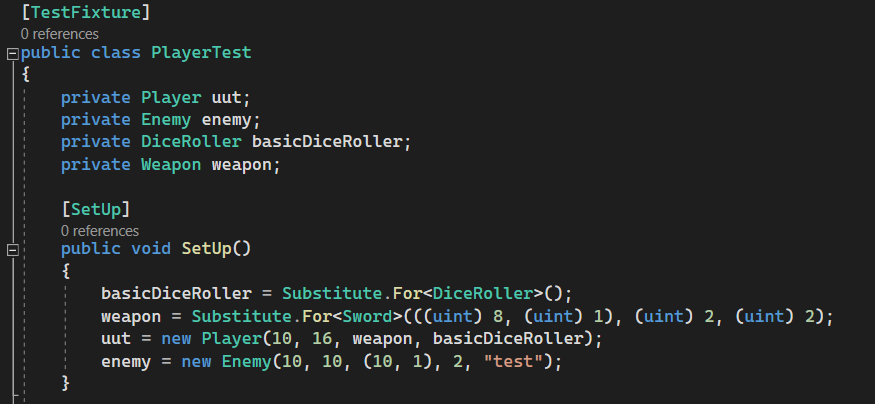
\includegraphics[scale=0.5]{02-Body/Images/Mocks_And_Dependency_Injection.png}
  \label{fig:mock}
\end{figure}

\begin{figure}[h]
  \centering
  \caption{Demonstration Af hvordan mocks kan bruges til at teste specifikke scenarier}
  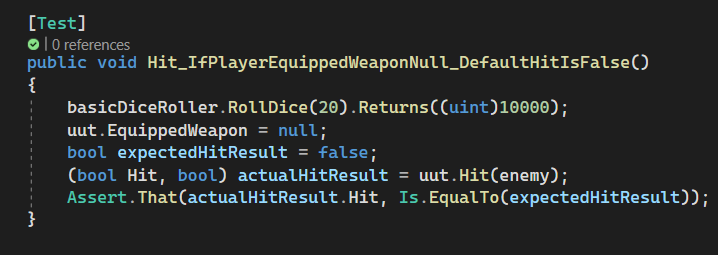
\includegraphics[scale=0.5]{02-Body/Images/UseOfMocks.png}
  \label{fig:MockUse}
\end{figure}


\newpage
